\documentclass[12pt]{third-rep}

%% Any characters from a % to the end of line are comments.

%% The third-rep class and this starter kit were written by 
%% Graham Gough <graham@cs.man.ac.uk>
%% If you have any comments or questions regarding this document,
%% please post them to the local newsgroup man.cs.tex.

%% This skeleton report is organised as a master file called
%% report.tex which then includes files for individual parts including
%% abstract.tex, chapter1.tex, chapter2.tex, chapter3.tex and
%% appendix1.tex.  

%% The third-rep style is a locally created style based on the
%% standard LaTeX report style. If you really want to have a look at
%% it, its source can be found in
%% /usr/local/share/texmf/tex/latex/mancs/third-rep.cls
%%
%% More information about LaTeX in general and the local setup in
%% particular can be found on the web at 
%% http://csis.cs.manchester.ac.uk/software/contrib/latex
%%
%%%%%%%%%%%%%%%%%%%%%%%%%%%%%%%%%%%%%%%%%%%%%%%%%%%%%%%%%%%%%%%%%%%%%%%%
%%
%% This is an example of how you load extra packages.
%% Some packages are already loaded in the third-rep class

%%\usepackage{url} % typeset URL's sensibly

\usepackage{pslatex} % Use Postscript fonts
\usepackage{graphicx}
\graphicspath{ {images/} }

%% The best way to latex just one chapter is to uncomment lines such as
%% the next:
%\includeonly{chapter1}

%% This defines the title (the \\ forces a line break)
\title{Visualisation of Allergy\\
  Hotspots}
%% and author
\author{Nick Burrell}
%% and supervisor
\supervisor{Dr. Andy Carpenter}
%% and the year of the report
\reportyear{2017}

%% this defines the file that contains the text of the abstract, there
%% must be one of these by the time you submit your report.
\abstractfile{abstract.tex}

%% this defines the file that contains the acknowledgements (it can be
%% omitted if you don't feel like thanking anyone
\thanksfile{merci.tex}

%% Uncomment the following lines if you want to include the date as a
%% header in draft versions. See the documentation for fancyhdr for
%% more ways of modifying headers (texdoc fancyhdr will show you the
%% docs) 

\usepackage{fancyhdr}
\pagestyle{fancy}
\lhead{}  % left head
\chead{Draft: \today} % centre head
\lfoot{}
\cfoot{\thepage}
\rfoot{}

%% The following line sets up the use of PostScript fonts rather
%% than the standard bitmapped fonts.
\usepackage{pslatex}

%% Uncomment the following line if you want to change the name of the
%% Bibliography to References
%\renewcommand{\bibname}{References}

\usepackage{listings}

%% End of preamble, the actual document starts here
%%

\begin{document}

%% This actually creates the title and abstract pages
\dotitleandabstract

%% Generate contents etc
\tableofcontents
\listoffigures
\listoftables

%% These include the actual text
\chapter{Introduction}
\label{cha:intro}

I will briefly explain my motivation for this project, my initial aims also provide an overview of what you will read in this report.

\section{Motivation} 
I have a long history with allergies. As far back as I can remember I have suffered from allergy symptoms ranging from waking up with gummy eyes to having a permanently sealed nose and tight chest. I've had little luck with medication so I usually end up trying to change my environment to limit the number of allergens with an air filter. Even an industrial air filter does not provide much relief for me.\\

When I saw this project proposed by Dr Markel Vigo I knew it was for me. The challenge of trying to find potential causes for specific allergies was quite exciting. Not only would providing a means for identifying hotspots and their causes help the scientific community, it would also help me personally.\\

The majority of my previous programming experience has been with java within the school and C\# when working for companies outside of University. I quickly realised this project would have to be done using some kind of web technology, so the fact I had very little experience with this side of computer science, I decided it'd be a great opportunity to develop my skill sets to help my career.\\

\section{Aim}
\label{sec:aim}

I gave myself the following four main goals that I wanted Inhale to fulfil;

\begin{enumerate}
  \item Visualise hotspots
  \item Be user friendly
  \item Be useful for future users. Both general public and researchers.
  \item Be accessible
\end{enumerate}


The most emphasis was on the identification of allergy hotspots. I wanted a hotspot algorithm that was both valid and  powerful to be combined with a useful visualisation technique. As I want Inhale to be useful for the general public, it's important that the visualisation technique used both looks good and accurately displays the hotspots generated by the algorithm.\\

%% Before anything data related, explain hotspots

\section{Report Overview}

There are no hard to understand, advanced computer science algorithms or techniques used in this project. However, I do make some decisions that will require some background knowledge and context of the related subjects in order to fully understand my reasoning. So the second chapter will provide a brief history of allergies and how certain types of allergies are relevant to my project.\\

I'll talk about the structure and content of the datasets used throughout and cover what similar applications already exist.\\

Once the basics are understood, I will take the reader through the design decisions and implementation stages of Inhale in Chapters 3 and 4. I will go into some detail of the core processes, but nothing too heavy.\\

Chapter 5 will explain how I did my testing and how I interpreted the resulting heatmap displayed by Inhale. I'll show you some of the interesting hotspots and how I evaluated them.\\

I'll conclude the report with a summary of my personal experience developing Inhale and my findings using the final product.\\
    

\section{Software Environment}

My environment options for Inhale were to make a Desktop Application for either Windows or MacOS, website, mobile app or a web application.\\

I decided against making a desktop app for any platform as by going with this route it limits the number of users instantly. Whilst the last two versions of Windows make up around 65\% of the Desktop market, that's still a potential 35\% of users that are completely unable to use my software \cite{windows}. As this project is likely to be shown to potential employers, it would be nice to have it on a platform that is easier to setup and get running.\\

A mobile application was a strong contender, with 

\subsection{Occam}

Here is some more example text, showing various \LaTeX\ facilities
you may need.  The project was mostly programmed in
\textbf{Occam}~\cite{occam}.  (A citation has been created  here to an
entry in the bibliography at the end of the report. See
chapter~\ref{cha:bib} for more details on how to do this).

Note the way of getting boldface, \textit{textit} is used for italic.
\emph{emph} is used for emphasis and is the same as italic except when
already in italic.  Note the cross reference to the bibliography.
This is how you create a footnote: DMA\footnote{Direct Memory Access.
  Footnotes can stretch over more than one line if you have a lot to
  say, but be careful not to overdo them.}.

Here is a reference to a figure. See figure~\ref{pipeline}.
\begin{figure}[htbp]
  \centering
  \setlength{\unitlength}{0.0125in}
\begin{picture}(300,35)(60,730)
\thicklines
\put(340,750){\vector( 1, 0){ 20}}
\put( 80,740){\framebox(20,20){}}
\put( 60,750){\vector( 1, 0){ 20}}
\put(100,750){\vector( 1, 0){ 20}}
\put(120,740){\framebox(20,20){}}
\put(180,750){\vector( 1, 0){ 20}}
\put(200,740){\framebox(20,20){}}
\put(160,740){\framebox(20,20){}}
\put(140,750){\vector( 1, 0){ 20}}
\put(240,740){\framebox(20,20){}}
\put(220,750){\vector( 1, 0){ 20}}
\put(260,750){\vector( 1, 0){ 20}}
\put(280,740){\framebox(20,20){}}
\put(320,740){\framebox(20,20){}}
\put(300,750){\vector( 1, 0){ 20}}
\end{picture}

  \caption{A Pipeline of processors
    \label{pipeline}}           %  this label must appear after the
                                %  \caption, and before the end of the
                                %  figure
\end{figure}
The picture in this figure was created the hard way using the picture
facility of \LaTeX. It is \emph{much} easier to use \texttt{xfig}, as
described in section~\ref{sec:diagrams}.  Whatever its contents, a
figure `floats' to a `suitable' point in the text and is never split
across a page boundary. (\LaTeX's idea of what constitutes a suitable
point may not coincide with yours)


Now we have a verbatim environment; this is a useful way of including
snippits of program, printed in a fixed width font exactly as typed:

\begin{verbatim}
{{{ An example of some folds
...  This is some folded code
  {{{ This is another fold
  This is text within the fold that has now been
  opened so that the text can be read.
  }}}
}}}
\end{verbatim}

% Everything below here is commented material which is used by the
% emacs tex support system called auctex. If you're not an emacs user
% you can safely ignore it. If you do use emacs you should take a look
% at the local emacs or LaTeX WWW pages for more on emacs support for
% LaTeX.

% Local Variables:
% mode: latex
% TeX-master: "report"
% End:


\chapter{Background}
\label{cha:back}

In this chapter I will cover the context of my project to allow the reader to understand the more complex parts of the report to come. First I will explain the different symptoms of hay fever and how they might be caused by different allergens. I will then talk about the main dataset used throughout and how I interpreted the data to produce meaningful results.

\section{Seasonal Allergies}
A massive 44\% of Britons suffer from at least one allergy, the majority suffering from some form of a seasonal allergy \cite{mintelallergy}. Allergies are on the rise, even with modern allergy medication continuously improving \cite{mintelallergy}. It is clear that something needs to be done to help those who suffer.\\


\subsection{Asthma}
When talking about hay fever, most people assume that it only affects the nose. However, in a study by Eur Respir J, it was found that 20.4\% of allergy sufferers also self-reported suffering from asthma \cite{rhinitis}. By 2025, it is predicated that asthma will represent the most prevalent chronic childhood disease and result in one of the highest health care costs, primarily due to the need for ongoing treatment throughout the patients life \cite{childhood}. Despite many decades of research, we do not have a complete working solution to the problem. The best we can do is limit exposure, Inhale will help with this by highlighting areas with unusually high occurrences of particular symptoms.\\

Listed below are the main causes of allergy induced asthma, the effects of which can impact everyday life of the sufferer.\\


\begin{itemize}
  \item Allergens: including pollen, dust mites, animal fur ("dander") or feathers
  \item Airborne Irritants: including cigarette smoke, fumes and pollution
  \item Emotions: including stress or laughter
  \item Weather Conditions: including sudden changes in temperature, cold air, windy days, thunderstorms and hot, humid days
  \item Infections: particularly infections of the upper airways, such as colds and flu
\end{itemize}\begin{center}Adapted from \cite{urlasthmacauses}\end{center}

There is a large variety of factors contributing to allergy induced asthma. It would be impossible to cover all aspects of these in this report. I am going to focus on the effects of Airborne Irritants and Allergens.


\section{Datasets}

In this section, I will describe the structure and features of the datasets used by Inhale.\\

\subsection{Britain Breathing}

Britain Breathing is a Citizen Science project run by the British Society for Immunology, Royal Society of Biology and the University of Manchester Immunology Group, who conduct research into the causes and treatment of allergies. To aid their research, they collect data on seasonal allergies using a simple but effective mobile application available on the Android operating system. Their aim is to get allergy sufferers to submit their symptoms regularly so that they can build solutions to the problem.\\

When setting up the application, you are asked standard registration questions such as your age, gender, and whether you suffer from pre-existing allergy related issues such as asthma and hay fever. In everyday use of the Britain Breathing app you are asked to rate the severity of your allergy related symptoms on each day. You are also asked whether you have taken your allergy medication for that day. This data is collected along with your location to be stored by Britain Breathing.

\begin{figure}[H]
\begin{center}
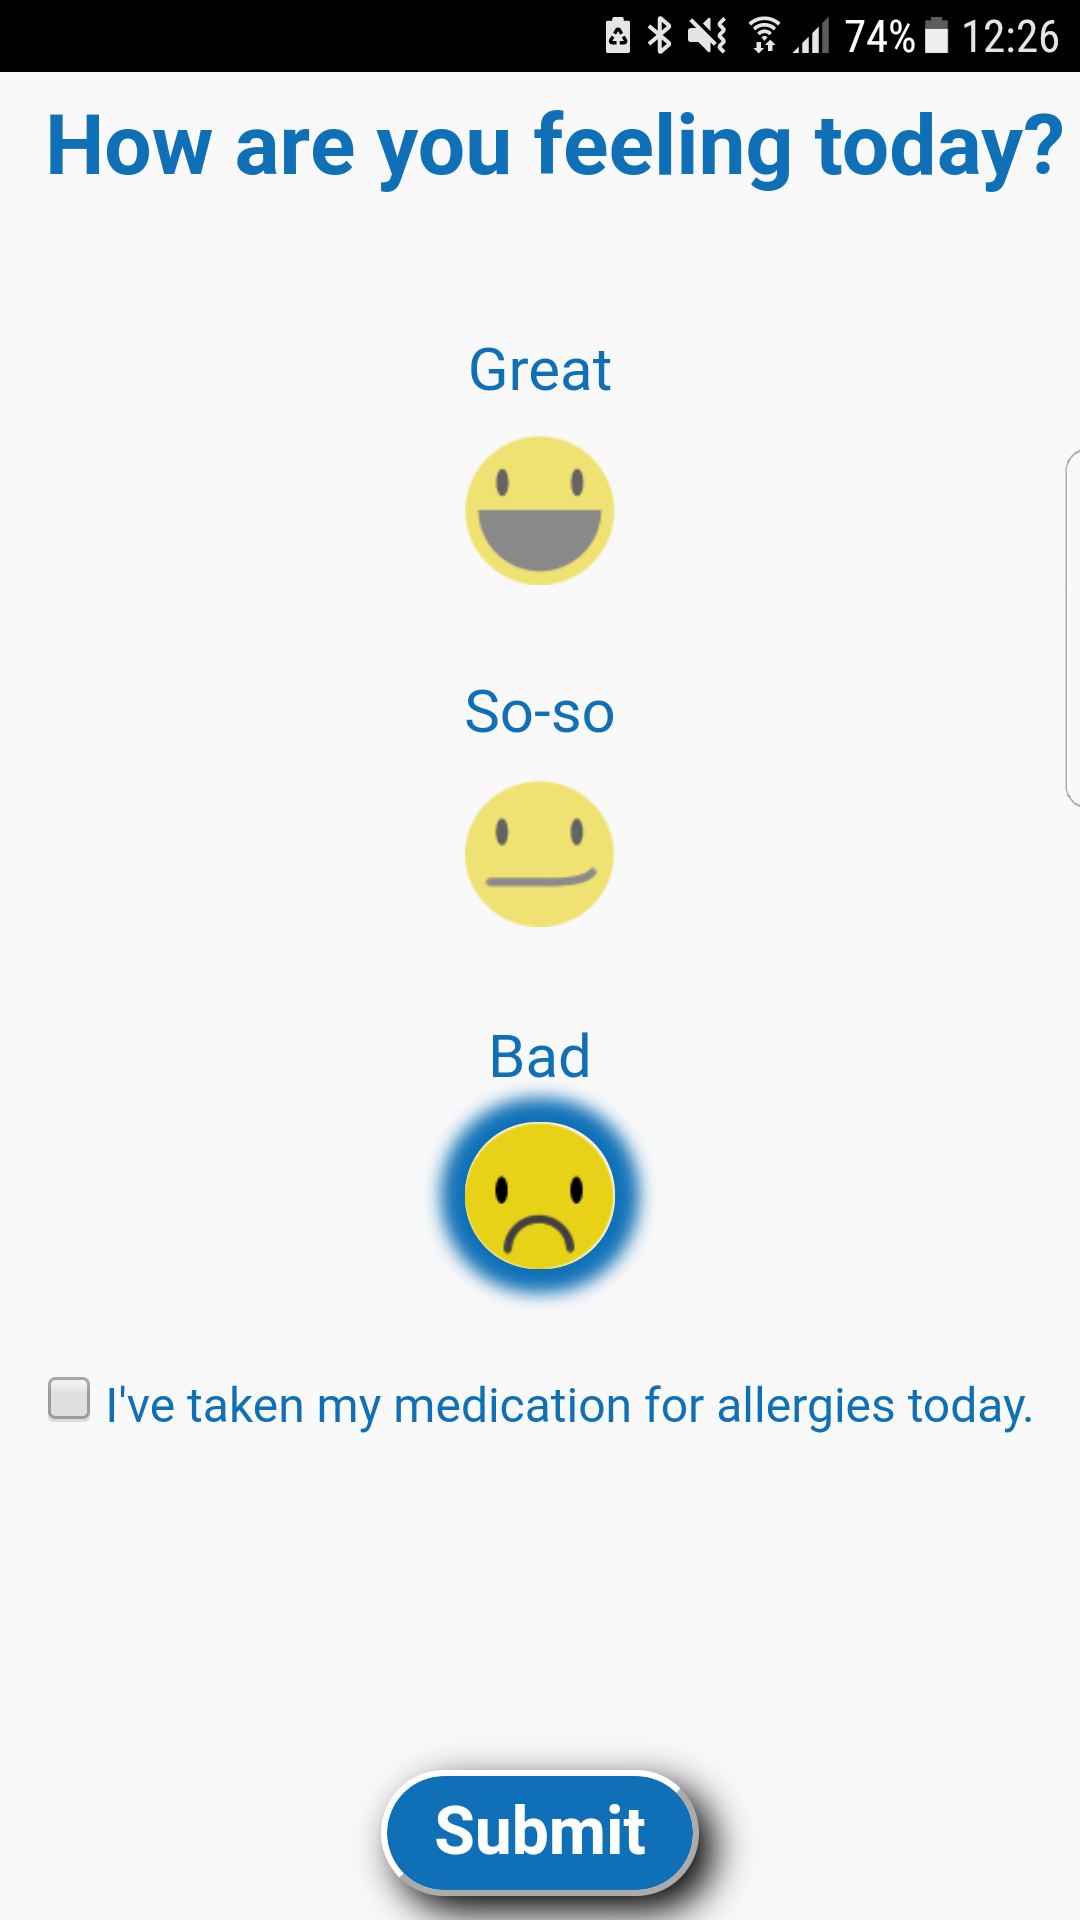
\includegraphics[width=6cm, height=8cm]{bbapp}
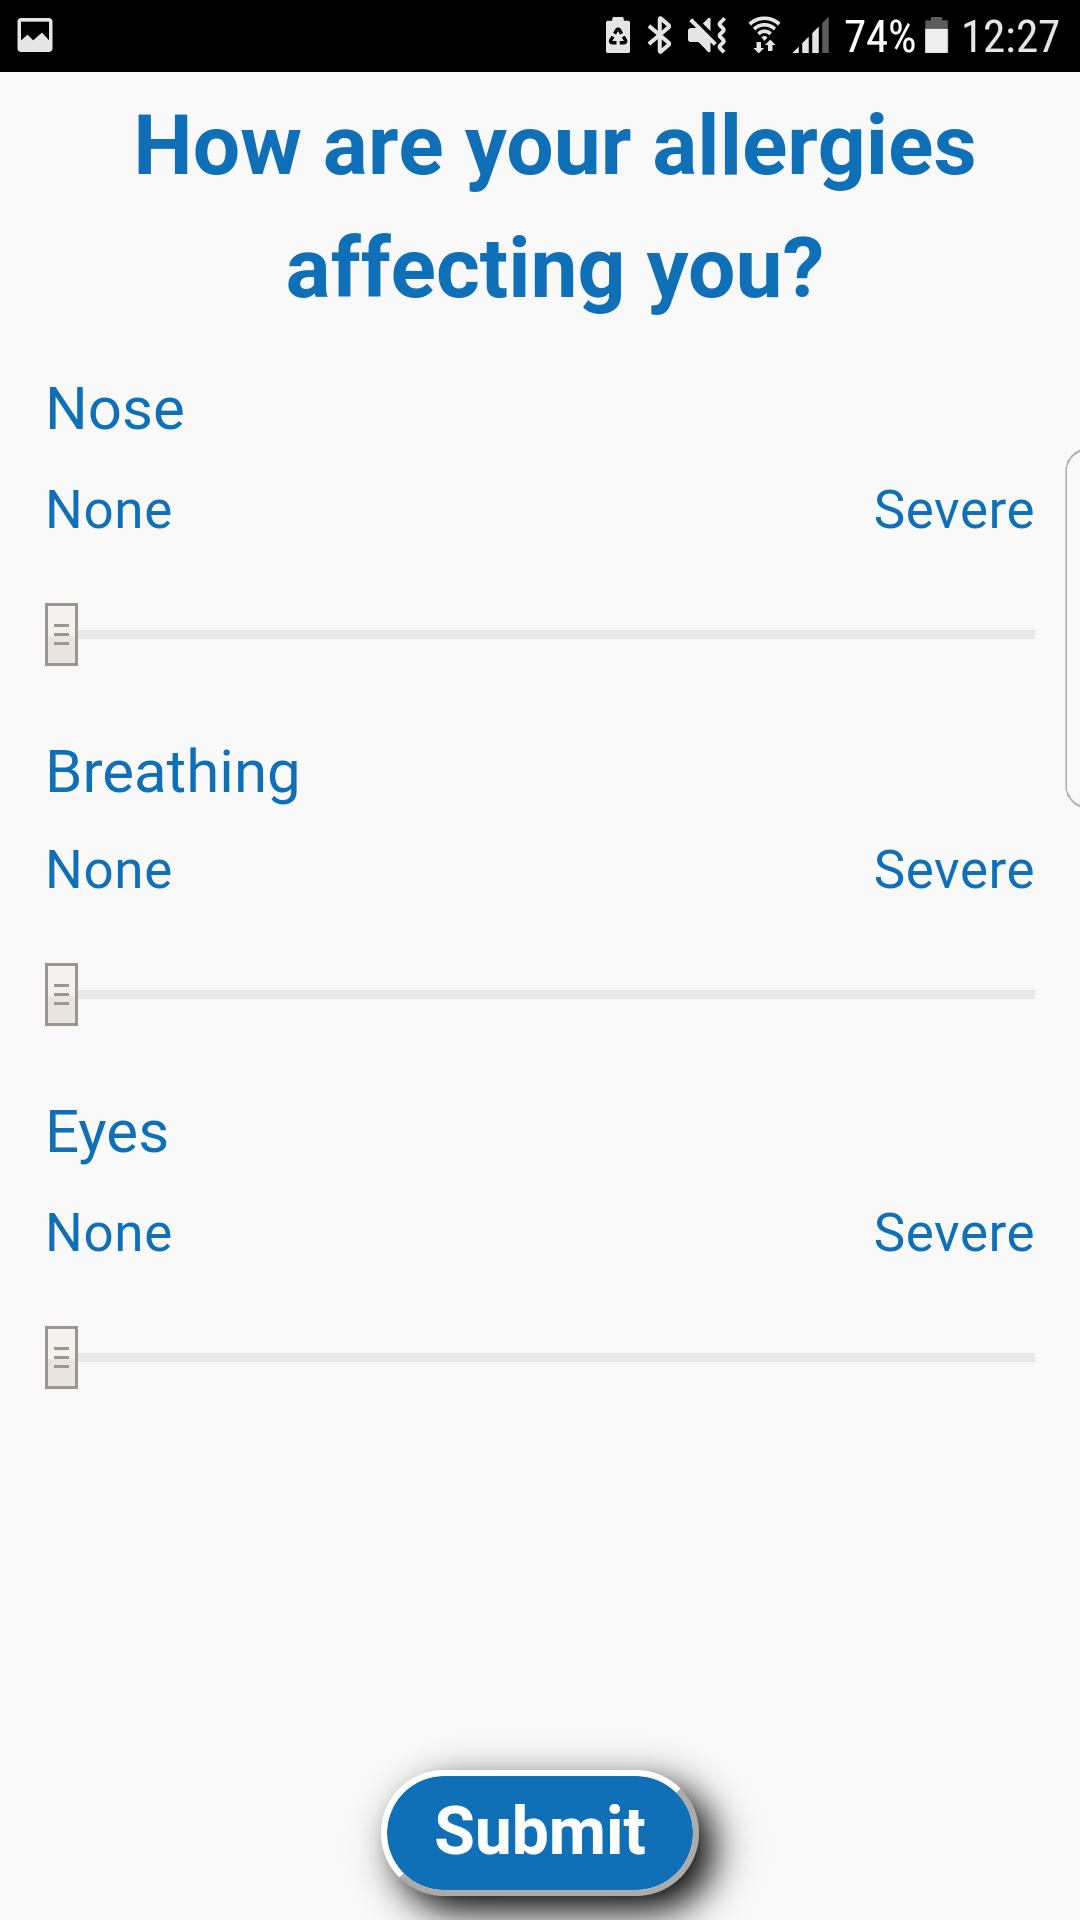
\includegraphics[width=6cm, height=8cm]{bbapp2}
\caption{Screenshots of the data collection screen on the Britain Breathing Android app}
\label{fig:bbscrn}
\end{center}
\end{figure}

Dr Vigo works with the Britain Breathing project, and was kind enough to provide me with their dataset from September 2016. This dataset contains 18,386 records from all over the UK. The data contains values corresponding to the questions asked in the application. They also ask whether or not the user has taken their medication today, this field is particularly useful as it can be used as a multiplier. If someone has severe nose, eye and breathing symptoms and they have taken their medication, then this should be expressed in the final visualisation as they're clearly being exposed to a significant amount of allergens.\\% avoid 'obviously', rephrase

The dataset covers nose, eye and breathing symptoms, see Table \ref{bbdatatable}. As these parts of the body are all interlinked in very close proximity, it makes sense to try to combine them. In Section \ref{sec:anal}, I will go into more detail as to how I combine these problematic areas into one value that summarises them.\\


\begin{table}[H]
\begin{center}
\begin{tabular}{|c|c|c|c|c|c|c|c|c|c}\hline\hline
Breathing&Eyes&How Feeling&Nose&Taken Meds&Asthma&Hay Fever&Latitude&Longitude\\\hline
0&0&0&0&1&1&0&54.10&-2.39\\
3&0&2&3&1&1&1&53.89&-2.79\\
3&1&0&3&1&1&1&53.24&-2.34\\\hline\hline
\end{tabular}
\end{center}
\caption{A Simplified sample of the 18,386 record Britain Breathing dataset}
\label{bbdatatable}
\end{table}

The Britain Breathing dataset will be the base for the entire project. Most of my time was spent with this set establishing a good hotspot identification algorithm and presenting it on a map.

\subsection{Other Datasets}

Whilst early testing and development involved many datasets, I decided on two main sets to use for comparison to the Britain Breathing dataset.\\

The data.gov website provides counts for Road Traffic data available for public use. The set contains 750,000 entries from major road traffic counts at locations all over the UK. They give a location of the Centre Point of the count, that is, where the counter was when recording the traffic. The northmost and southmost junctions on either side of the Centre Point. For each record, the counts for different vehicle types are given. Vehicles are categorised into Cars, Buses, Large Goods Vehicles (LGV), Heavy Goods Vehicle Rigid axle (HGVRx) and HGVAx for articulated HGV's where x is the number of axles of the HGV. See Table \ref{RoadTrafficData} for a simplified version of the dataset.\\


\begin{table}[H]
\begin{center}
\begin{tabular}{|c|c|c|c|c|c|c|c|c|c|c|}\hline\hline
S Ref E&S REF N&Road&A REF E&A REF N&Hour&CAR&BUS&LGV&HGVR2&...\\\hline
90200&10585&A3112&90320&10530&7&24&6&13&5&...\\
380927&405391&M60&382819&405920&15&7642&18&300&64&...\\
380927&405391&M60&382819&405920&17&10042&32&654&103&...\\\hline\hline
\end{tabular}
\caption{Simplified example of the 750,000 record Road Traffic dataset. 20 columns have been removed for viewing purposes.}\label{RoadTrafficData}
\end{center}
\end{table}

The second set used is a dataset of the large urban areas in the UK. The data is fairly simple consisting of a location feature in the form of a Latitude and Longitude and a name for the area. I used this dataset as a guide in the hope that it might help highlight interesting areas. Areas that are not in a large urban area but are indicated as a hotspot should be investigated further. However, it is not used for any particular research benefit, nor is it used to draw any conclusions.\\

\section{Using Datasets}

The number of people suffering from allergic rhinitis is rising, and whilst increased carbon emissions and global warming are lengthening the pollen season, there are not significantly more pollen producing plants and trees year on year \cite{co2pollen, allergyrising}.\\

The main pollutants emitted by combustion engine vehicles are:

\begin{itemize}
    \item CO
    \item $SO_2$
    \item $NO_x$
\end{itemize}

\begin{center}
Adapated from \cite{vehcemis}
\end{center}

It has been proven that these pollutants, whilst perhaps not associated with hay fever symptoms by most, are actually all directly associated with allergic rhinitis\cite{airPollution}. With this in mind, we can compare the Road Traffic dataset with the Britain Breathing dataset on the same map to try and find some correlation.\\

\section{Existing Applications}
\label{sec:diagrams}

There are few directly relevant applications. The reason for this is that in order to produce a meaningful application a well-formed dataset is required. In order for a dataset to be relevant, it needs to be of a reasonable size, have a good range of locations and a diverse demographic. Without collecting data from the people directly affected by allergens it's not possible to make educated conclusions on allergy hotspots. Currently there are no existing applications that satisfy this criteria.\\

\subsection{Britain Breathing}
Britain Breathing have a Data Visualiser on their website. It provides a simple display of the allergy data collected in a particular data range, for a particular data value. At the time of writing this report, the Visualiser is not working so I can only display a screenshot of the interface without the map containing the visualisation.

\begin{figure}[H]
\begin{center}
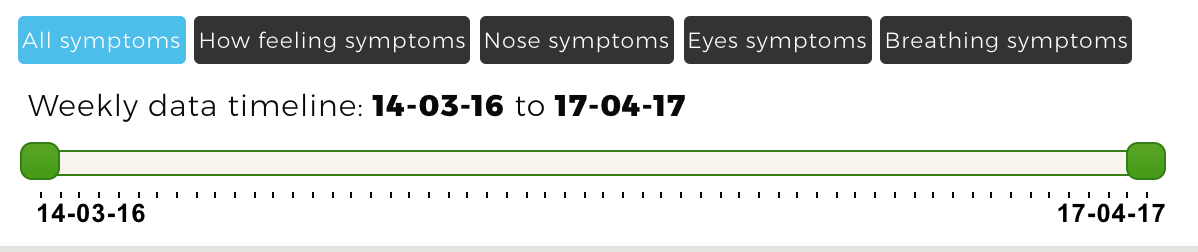
\includegraphics[width=0.75\textwidth]{bbvisinterface}
\caption{Britain Breathing Visualiser Interface}
\end{center}
\end{figure}

\subsection{Pollen forecast}

The most comparable applications to Inhale are pollen forecast services such as Pollen.com's allergy forecast map. As the name suggests it only displays pollen forecasts, not allergy symptoms. Whilst pollen is a major contributor to allergy symptoms, it needs to be combined with the other problematic allergens to be make credible conclusions.\\

Therefore, without the data from an organisation like Britain Breathing, it is not possible to make a comparable application.

\begin{figure}[H]
\begin{center}
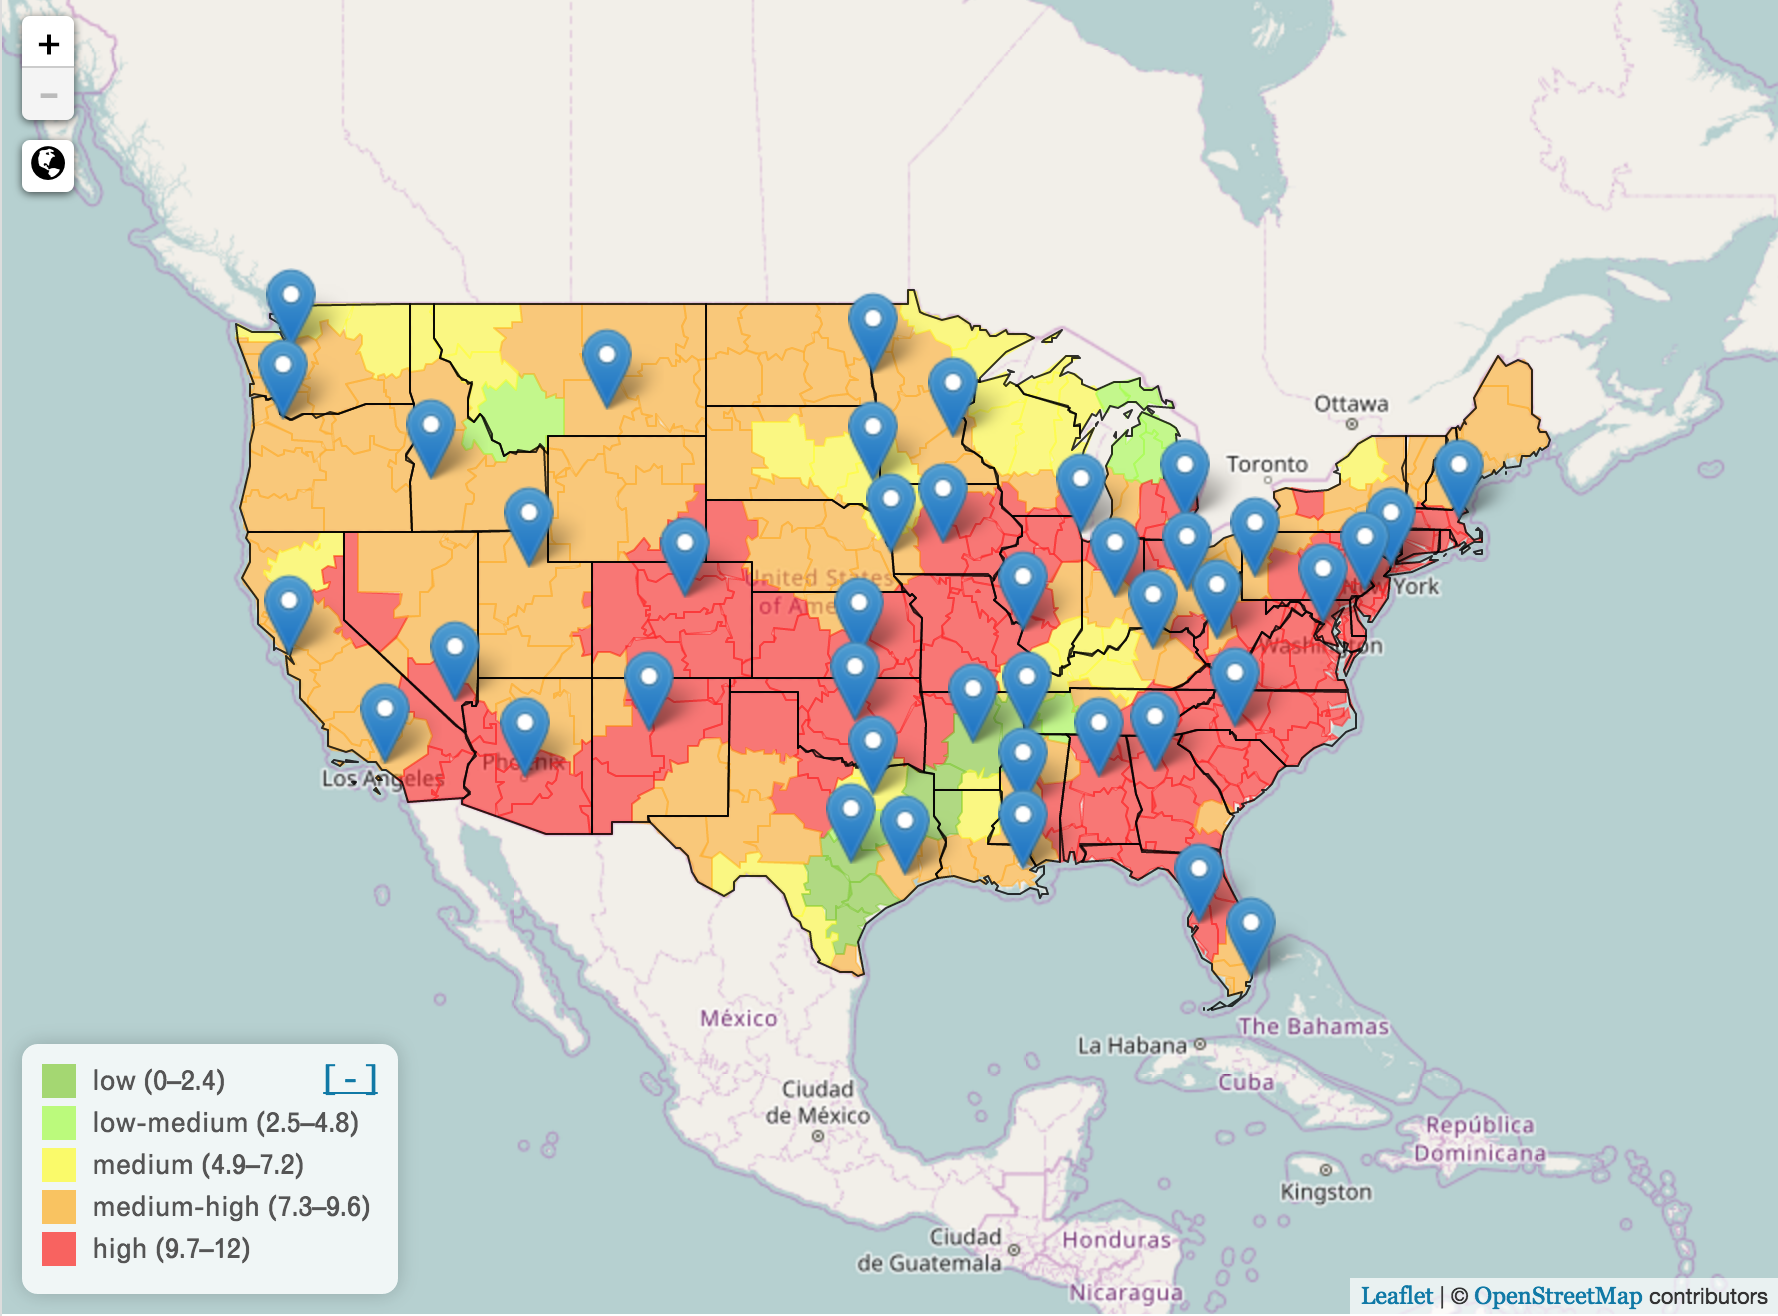
\includegraphics[width=0.75\textwidth]{pollenforecast}
\caption{Pollen.com Allergy Forecast Map}
\end{center}
\end{figure}

\section{Remarks}

After looking at many other mapping applications, it has become clear that using the standard Marker to represent points on a map can be used if and only if there are a very low density of points. Any other scenario results in a map that is totally incomprehensible.

\begin{figure}[H]
\centering

\includegraphics[width=0.05\textwidth]{marker}
\caption{Marker}\label{fig:marker}
\end{figure}
\chapter{Design}
In this Design section, I'll explain how and why I chose the Software Architecture I did, and what tools I used to develop Inhale. I won't go into the details, just enough so that the Design choices are justified.

\section{Architecture Choice}

As all of the datasets I'll be using for Inhale will be geographical datasets, meaning they all have a location attribute, it is imperative that they are displayed on a map. Trying to make any sense of a geographical dataset without seeing it on a familiar map is nearly impossible.\\



\subsection{ArcGIS by Esri}

ArcGIS is an incredibly powerful contextual tool for mapping and spatial reasoning. Its features are so well made that I initially thought using some form of this software would be the only viable solution. It allows you to produce good-looking, user-friendly maps with very few lines of code. It  also provides a mass of data processing tools, including hotspots analysis and data correlation.\\

Ultimately, I chose not to go with ArcGIS because it costs around £1200 for one license. However I also wanted to implement my own algorithms, using ArcGIS would not leave me with much to implement, and after all, this is a computer science project. I can see how ArcGIS could be incredibly useful for businesses and marketing/pr.

\subsection{Desktop Mapping Tools}

There are various desktop mapping tools available, even open source options that have a good variety of features. The main issue with this style of mapping software is it's expandability, accessibility and familiarity.\\

Although tools like MapSphere allow you to make 3rd party plugins to expand the standard application with your own features, the features you're given access to when developing those plugins is quite limited. I want the scope to be able to implement whatever I want. 
Being a desktop application, you're cutting down your potential users, not everyone wants to download an application, it feels too heavy and sluggish for modern users when you can access perfectly able maps from our pockets in the form of smartphone apps and websites. I wanted Inhale to be familiar to the user, I wanted to use controls people are used to using from their everyday use of Google Maps, Waze etc. All of the free desktop applications I tried felt very old and sluggish.\\

\subsection{Google Maps}

After playing around with ArcGIS and desktop mapping tools, I was aiming more towards a solution involving a dynamic mapping provider. Google Maps does not need an introduction. Google have an API that allows developers to implement their own features, toolbars and map tiles. The API can provide maps on various platforms from Android, iOS, javascript and more.\\

The biggest draw towards Google Maps is their places API, it allows you to search for establishments, geographic locations, or prominent points of interest in a well defined area around a point \cite{googlePlaces}. This would be incredibly useful for Inhale as once a hotspot is identified, you could search for nearby places that may be contributing to the symptoms in that area. The only problem here is that it's very difficult to implement a general approach to getting nearbly places that have an affect. Google sort their places by type, the types are aimed towards general public use. They're in categories such as art gallery, bakery, bank, pharmacy, hospital. Whilst it could be argued that you could count the number of commercial premises nearby, but I don't believe this is enough to provide any sort of answer to allergy hotspots.\\

Google Map's main downfall is the lack of customisability, it lacks some features compared to other mapping options.

If Google ever increase the number of categories, or maybe include more general options such as "industrial" or "factory" then it would definitely be the best option.\\

\subsection{Leaflet}

Leaflet is a javascript library for mobile-friendly interactive apps \cite{leaflet}. Leaflet is comparable to Google Maps in that it has many of the same features. Leaflet is open source, has many third party plugins with a thriving community contributing daily towards building a versatile dynamic mapping tool.\\

I decided to use Leaflet for my project as it is the most customisable of all the options investigated so far. It allows me to develop whatever I want to, and make my map look exactly how I want.\\

One particular third party plugin that drew me towards Leaflet was heatmap.js. Heatmaps seem like the best way to present the results of a hotspot identification algorithm. After testing the built-in Google Maps heatmap, I was disappointed with both the speed and custom options available.\\

Leaflet was chosen because it can be used in a web format, it is very customisable and it has a lively community contributing to features all the time. I would be easy to add necessary features further down the line.

\section{Leaflet}

Talk about how you use leaflet.

So, once the data is ready to be displayed, you pass to leaflet as heatmap layer.

Deals with layers

Tiles - Simplicity - familiarity

\section{Development Tools}

Tableau

Chrome dev tools
\chapter{Implementation}
\label{cha:impl}

Chapter 4

\section{Pre-Processing}

Figure \ref{bbdatatable} shows the raw format of the Britain Breathing dataset. There are a few procedures that need doing before it can be used in a hotspot identification algorithm. Before I had a web page running with the capability of displaying geographical data I relied on Tableau to visualise and alter all datasets.\\ 

The Britain Breathing dataset in it's raw format contained entries from all over the world. I could have decided to leave them on as I could centre the map on the UK so only those who where curious enough to pan around the rest of the globe would see these extra points. But that's more of a novel thing. At the time of pre-processing, I thought the extra points might affect some of the hotspot algorithm calculations such as global averages so I decided to remove all points that are not on mainland UK or in Northern and the Republic of Ireland.\\

\begin{figure}[H]
\begin{center}
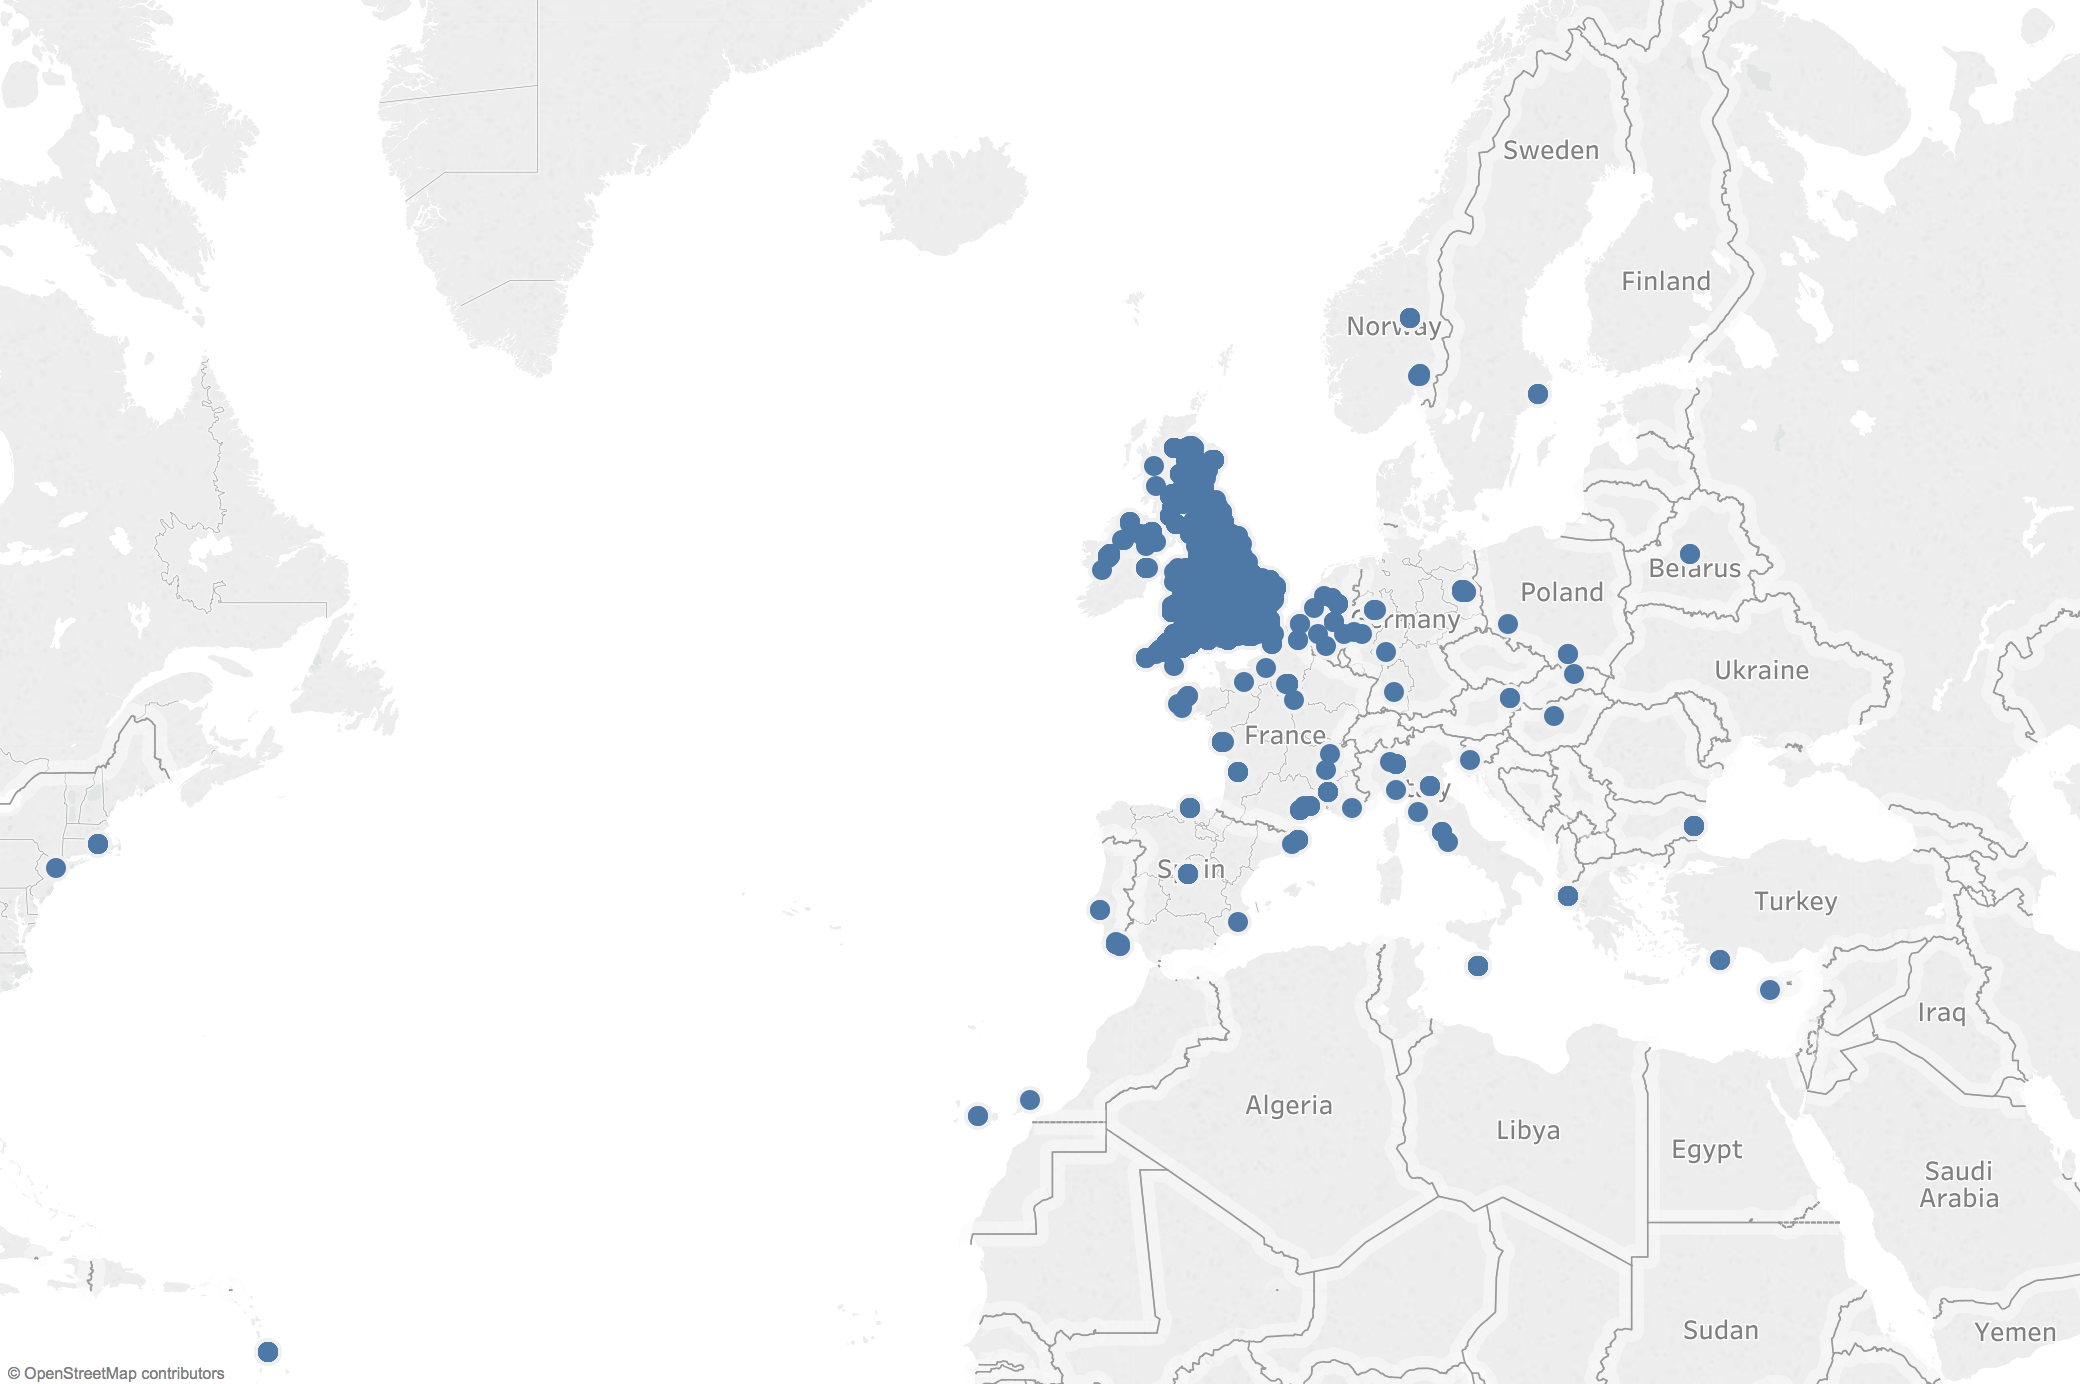
\includegraphics[width=0.75\textwidth]{tableuaeverywhere}
\caption{Britain Breathing dataset before processing}
\label{fig:RTv1}
\end{center}
\end{figure}

Approximately 2.7\% of entries had a null value for one of the attributes. 96\% of these nulls were  whether or not the user had existing hay fever or asthma, I decided to remove each of these records entirely, I could also have decided set the attribute to 0 or 1 but I wanted to avoid fabricating data to keep any conclusions made using the data valid.\\

Whilst using Tableau to visualise the data in the early stages of development I noticed there were a few clusters of points in virtually the same place. For example, there is a user in the north of Scotland who used the app at times multiple times a day to record her allergy symptoms. This resulted a fairly large set of results for a very sparsely populated area. I decided to remove most of the results for this person as the area was identified as a hotspot. I think there could be arguments for keeping the data but I don't think that allowing one persons enthusiasm to track her allergy problems makes sense for a project aimed at producing results that could be used to aid research.\\

Once the data has been improved from its raw format, it is stored on the server as a .JSON file. I decided against using a database to store my datasets as I wanted to avoid having to convert to and from JSON. The end application ended up being rather CPU intensive so this decision turned out very well.

\subsection{Road Traffic}

The Road Traffic dataset in its raw format was far from being usable.\\

As you can see from figure \ref{fig:rt} the first version of the Road Traffic dataset was way too dense. I needed the dataset to be able to be displayed with the heatmap generated from the Britain Breathing dataset to be visible behind the Road Traffic data in order to compare the two. There were too many roads of very short spans cluttering the view of the heatmap.\\

\begin{figure}[H]
\begin{center}
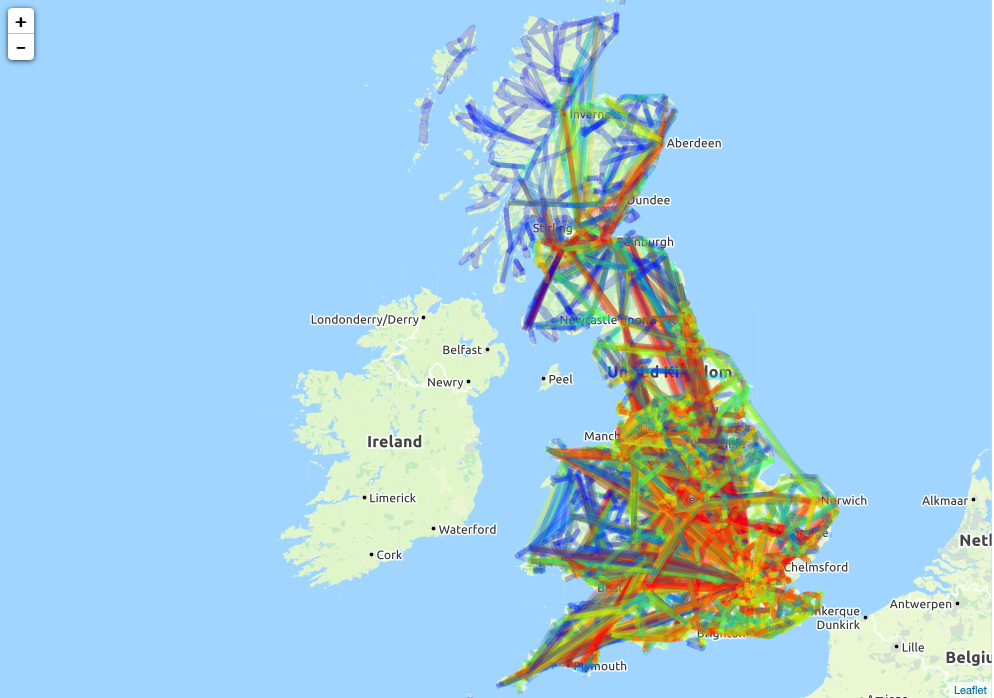
\includegraphics[width=0.75\textwidth]{RoadTrafficv1}
\caption{First attempt at displaying the Road Traffic data. There's a bit much going on here.}
\label{fig:rt}
\end{center}
\end{figure}

Upon zooming in and inspecting the data I also found that some roads were stored incorrectly in the dataset. Around 10 roads were stored as having their junction before and junction after being the ends of the road. Roads like the A1 can be as long as 396 miles so errors can cause big problems \cite{longestRoad}. In the case of the A1, the entire road was displayed as a deep red indicating a high volume of traffic. For the majority of the A1, this would be true but there are areas of the road that are not particularly busy so they're being wrongly represented. \\

I created a java program to process the data before being stored on the server. Java was chosen purely because I have most experience with it and I knew exactly how to read and write files, making it a good choice for pre-processing the Road Traffic data. For each entry, counts are discarded if the length of the distance between the junction before and the junction after is longer than 200km or if the road is shorter than 5km and has a density in the lower 5\% of the data. Removing the smaller roads like this removes the mess of small roads with negligible traffic in places like the north of Scotland. These roads don't provide much information and therefore do not help to find hotspots, they just make the map look cluttered.\\

\subsection{Analysis Field}

The Britain Breathing dataset has many attributes that are relevant to allergy symptoms.\\

Figure \ref{table:bbdata} : Britain Breathing Dataset Allergy Related Attributes. 13 attributes removed for simplicity.\\\label{table:bbdata}
\begin{tabular}{|c|c|c|c|}\hline\hline
Attribute&Represents&Range&Range Description\\\hline
how\_feeling&General well-being of the person&0..2&0 Best, 2 Worst\\
breathing&Condition of lungs and trachea&0..2&0 Best, 2 Worst\\
eyes&Condition of the eyes&0..2&0 Best, 2 Worst\\
nose&Condition of the nose&0..2&0 Best, 2 Worst\\
hayfever&Suffers from hay fever&0..1&0 no, 1 yes\\
asthma&Suffers from asthma&0..1&0 no, 1 yes\\
taken\_meds\_today&Taken allergy medication&0..1&0 no, 1 yes\\\hline\hline
\end{tabular}

All of the attributes in Figure \ref{table:bbdata} contribute to the overall severity of a persons allergy symptoms on any given day. In order to use with hotspot identification algorithms, I need a single attribute that is a summary of the others. I need to combine them all into one value that can be used to score a certain records Allergy Score, or more generically to fit the Road Traffic dataset too, the Analysis Field.\\

In the development of the Analysis Field for the Britain Breathing dataset, I made some initial judgements and then adjusted the parameters with some trial and improvement. The Analysis field needs to be a summary of the others. Keeping this in mind, I assigned a high priority to the how\_feeling attribute as it itself is a summary of the persons general allergy related feeling. I then assigned breathing, nose and eyes with roughly similar weightings. I used the taken\_medication\_today as a multiplier for the breathing, nose and eye symptoms using the logic that if a person has taken their medication and is still suffering, then they should score higher than someone with the same values for the other attributes but has not taken their medication. hayfever and asthma attributes are used, but do not have much of an effect on the Analysis Field.\\

\begin{myequation2}%
Analysis Field (AF) = 2*(how\_feeling*(0.5*nose + 0.3*eyes + 0.3*breathing))
\end{myequation2}
\begin{myequation2}%
+ (taken\_meds\_today*(nose + eyes + breathing)) + asthma + hayfever
\end{myequation2}

The above formula is used to calculate the Analysis field in the final version of Inhale. It seems to work well, I'm happy it uses a wide spread of attributes but still focuses on the main four; how\_feeling, nose, breathing and eyes.\\

The Analysis field for the Road Traffic dataset was simpler. To keep the field relevant to allergies, I decided to focus on the emissions from vehicles on that road per hour. At first I simply found that the average $CO_2$ emissions for a combustion engine vehicle was 411 g/mile or 274g/km and I multiplied the total traffic count by this value \cite{trafficemiss}. The traffic counts were not anywhere near perfectly distributed. Different roads had very different distributions of vehicle types. For example, the two main corridors between the North and South of England, the M6 on the East and the A1 on the West both had far higher percentages of HGV type vehicles than average.\\

With the disparity in vehicle distribution in mind, I found the average vehicle emissions for each vehicle type instead. Then simply created the Analysis Field as below.

\begin{myequation2}%
Analysis Field (AF) = \sum_{vt=1}^n VehicleCount * VehicleTypeEmissions
\end{myequation2}

As previously mentioned, the dataset is not entirely consistent with its junctions before and after the counting point. Ideally, I'd use the vehicle emissions per km and multiply that by the distance between the junction before and after to get a total emission value for the vehicle. Not only would this not be possible due to the problems in the dataset, but it would also produce useless results. It doesn't matter how far a vehicle has travelled on its way to you, only the distance it has travelled in a small radius around you should be considered as this is the area in which its emissions can reach affect you.\\

As a compromise, I simply used the g/km value without taking into account the actual number of km used. This could maybe be improved by calculating the distance of the road that is within x km of the user.

\section{Heatmap Generation}

Once the data is in a useable format and condition, I need to display that data on a map. In this section will explain the steps taken to get to point where I have a allergy symptom hotspot represented as a heatmap using Leaflet.\\

The Britain Breathing JSON file is loaded from the server. An instance of a HotspotArray is instantiated with parameters including x and y values for the dimension of the desired map resolution. The resolution values are used to create a two dimensional array with sizes [x][y]. This array is used to divide the area of the UK into distinct square areas. See figure \ref{fig:hh} for a small scale example.

\begin{figure}[H]
\begin{center}
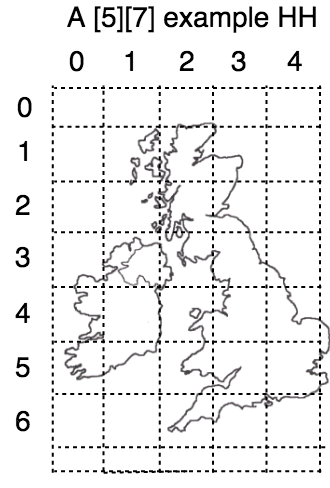
\includegraphics[width=0.4\textwidth]{hh5x7}
\caption{A [5][7] resolution example}
\label{fig:hh}
\end{center}
\end{figure}

By default, I used a 500 by 500 resolution as I found this gives enough of a resolution so that you can't see the square boundaries at any zoom level but also keeps the map easy to use in calculations. The alternative here would have been to use something like the UK Council boundaries, but I didn't like how they looked on the map. This was mainly due to the fact that dividing the map by Councils meant that you don't get precise enough information on specific allergy symptoms hotspots. A hotspot in a City such as Inverness would cause a massive area including tiny three or four house villages in the middle of the Scottish highlands to be indicated as being a "hotspot".\\

For each entry in the processed dataset;

\begin{enumerate}
    \item Add entry to the Hotspot Array. The latitude and longitude of the entry is used to map to an index in the array. For example, a location in the top left of the map would map to [0][0], bottom right would map to [499][499] etc. 
    \item If there is already a value in the Hotspot Array, add to the total count and update the average for the square area. Otherwise, add to the total count and calculate average.
\end{enumerate}

The next step after filling the Hotspot Array with the data is to do some hotspot identification.

\subsection{Spatial Autocorrelation}

Determining if an area is a hotspot or not can be done using Spatial Autocorrelation (SA). SA is a way of giving a numerical value to the degree of which an area is similar to nearby areas \cite{autocor} . A high positive value indicates that an area has a statistically significant value when compared to its neighbours and should be indicated as a hotspot. A low positive or negative value indicates that it is likely that the value is randomly clustered. A high negative value shows a cluster of low values. See Figure \ref{fig:autocor2}\\

\begin{figure}[H]
\begin{center}
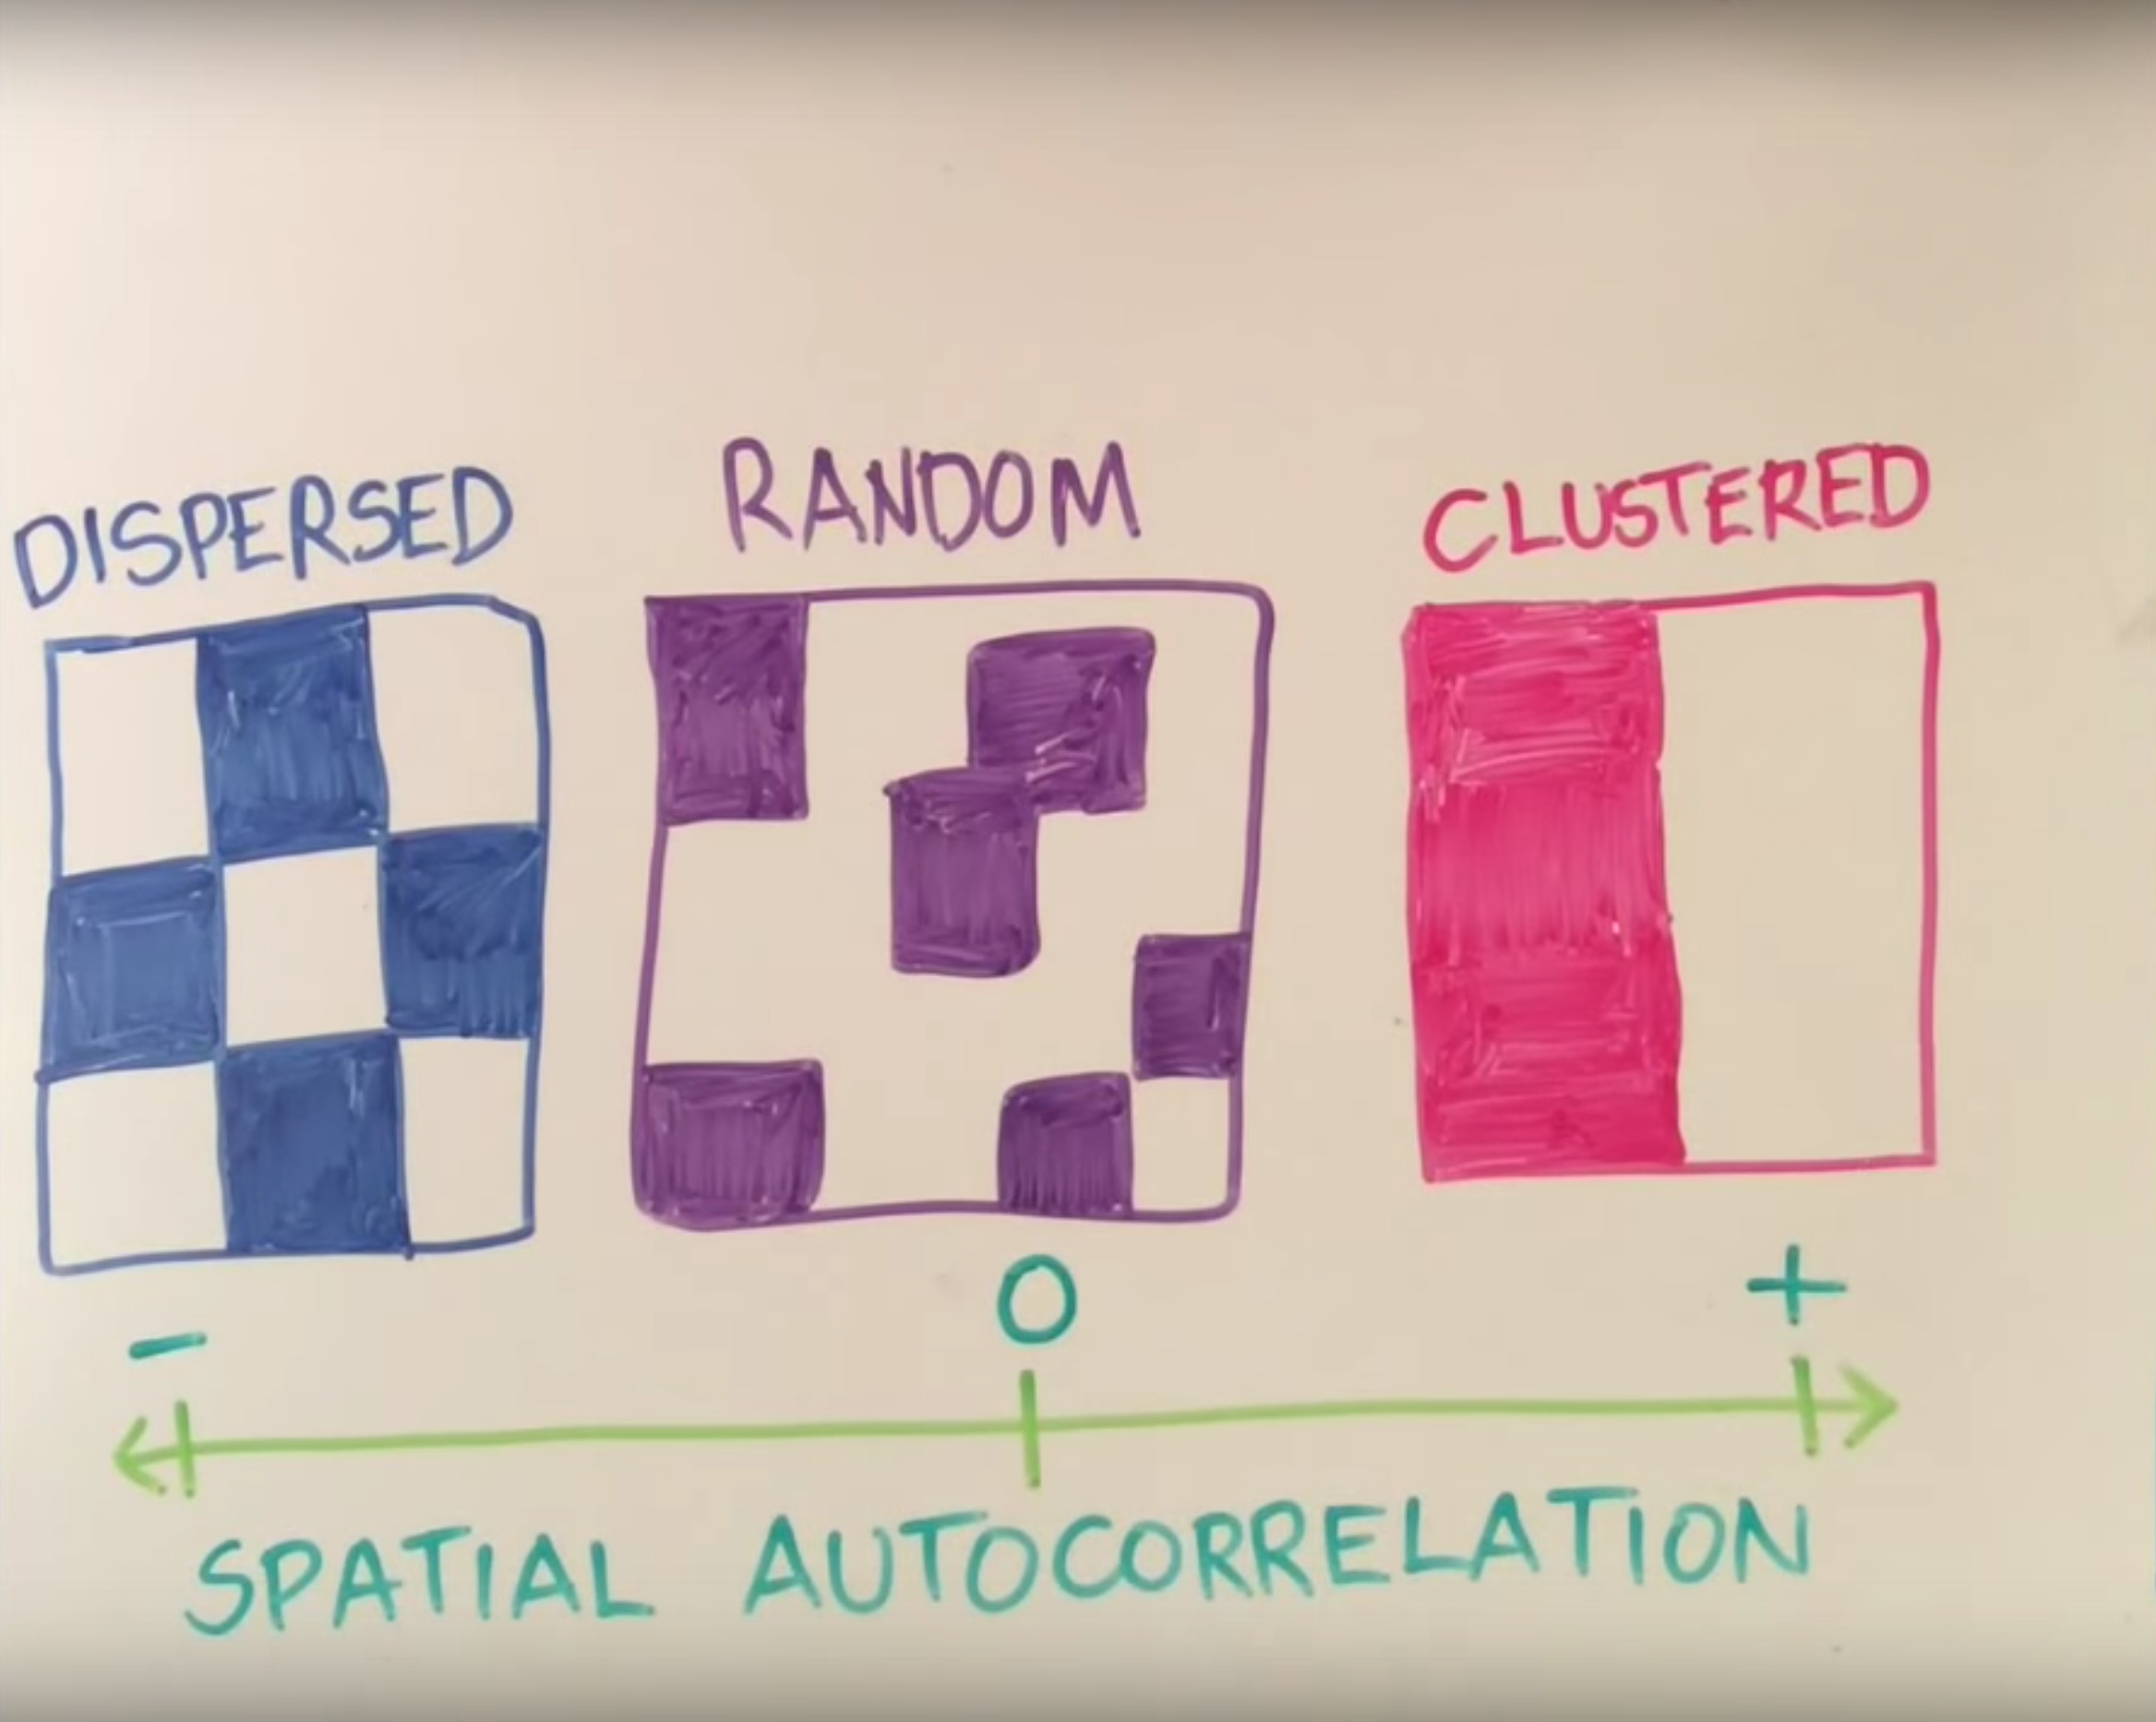
\includegraphics[width=0.8\textwidth]{autocor2}
\caption{Correlation Types}
\label{fig:autocor2}
\end{center}
\end{figure}

If an area has a high positive value then we can consider that area a hotspot. So if an area has lots of high positive values they should accumulate to generate a higher allergy symptom score. Equally, if an area has a few high positive values, a few small absolute values and a few large negative values, the algorithm should take this into account and not label the area as a hotspot.\\

An effective way of doing this is to take an average of the z-scores for the area. Then use the average in the heatmap.

\subsection{Distance Calculations}

Calculating the statistical significance of values, and whether or not they are related to nearby values involves calculating the distance between points.\\

There are many ways of calculating the distance between two dimensional points and it's not a particularly interesting topic so I'll keep it brief. I decided to use the Manhattan distance as shown below \ref{dia:manhat}.\\

$dist (x, y)  = \sqrt{\sum_{i=1}^n (x_i - y_i)^2 }$
\label{dia:manhat}

\subsection{Using distances}

The closer two points are, the more they will affect each other. It would not be correct to say that a cluster of allergy symptoms in Manchester should have any affect at all on those in Liverpool. So I need a way of using these distances to calculate how much to take the surrounding areas into account. Or as Waldo Tobler's first law of Geography puts it. "everything is related to everything else, but near things are more related than distant things." \cite{waldo}\\

As you know by now, the focus of this project is on the symptoms  of allergies. Most allergen producers do not have a method of mass dispersion. What I mean by that is they do not have a way of dispersing the produced allergens significant distances. Around 2km is normal, with the largest known distance being 21km \cite{pollenwr}. I can use this fact because I want to make sure that my hotspots are location specific and don't take into account the allergen producers over 20km because the chances are that allergens produced by them haven't reached the area.\\

The length of the entire UK is around 874 miles, with the length of the visible map in Inhale being 1000 miles. Divide this by 500 and you get 2 square miles per HotspotArray entry. This means that the average point in an area has a distance of 2 miles to the average point in the area directly to the left, right, up or down. When comparing to neighbouring areas, I want to consider the area directly next to the area in question, and maybe only very slightly consider the areas one square further than those, just to account for other types of allergens which may travel further.\\

I decided to use a inverse distance weighting with a strong fall off for neighbouring areas. See Figure \ref{table:dist} for the calculations used to determine the inverse distance function. I decided to use $\frac{1}{x^3}$ as it has the right amount of drop off for distances of 3 or more but still uses areas of distance two with a 12.5\% factor.\\ 

\begin{table}
\begin{center}
Figure \ref{table:dist} : Potential Inverse Distance Functions\\\label{table:dist}
\begin{tabular}{|c|c|c|c|}\hline\hline
x&$\mathbf{\frac{1}{x^2}}$&$\mathbf{\frac{1}{x^3}}$&$\mathbf{\frac{1}{x^4}}$\\\hline
1&1&1&1\\
2&0.25&0.125&0.0625\\
3&0.111&0.037&0123\\
4&0.0625&0.0156&0.0039\\\hline\hline
\end{tabular}
\end{center}
\end{table}


\subsection{Getis-Ord}

Getis-Ord Gi* is a spatial autocorrelation algorithm. I decided to use Getis-Ord Gi* as the alternative solutions tended not to include the feature being examined in the distance weightings. For this particular usage it is very important to include the immediate area when calculating z-scores as allergen dispersion distances are so small.

Here's the equation;

\begin{myequation}%
Gi^(*) = \frac{\sum_{j=1}^{n} w_{i,j}x_{j} - \overline{X} \sum_{j=1}^{n} w_{i,j}}{{S \sqrt{\frac{n \sum_{j=1}^{n} w^2_{i,j} - (\sum_{j=1}^{n} w_{i,j})^2}{n-1}}}}
\end{myequation}

In summary, it takes the Analysis Field and compares it to every other point on the map using the inverse distance function making sure that distant areas have less effect on the resulting value. This is then used to determine whether or not the area is locally statistically significant.

\subsection{Speed issues and the Solution}

When calculating the Getis-Ord Gi* values for each area in the 500 by 500 array, you need to calculate the distance between that area and every other area. This quickly becomes a large problem of scale $O(n^2)$. Even though the distance calculations are very fast, the total time to run the Getis-Ord calculations was 14 seconds. As Inhale is hosted online, users will be expecting a much faster, more fluid experience.\\

The Britain Breathing dataset is displayed by default every time you open the website. However, no changes are made to the data, the Getis-Ord calculations are stable so that the same input will always produce the same output so I can store the output from the Getis-Ord calculations so that I don't have to do them every time.\\

I implemented a cache system to speed up the process wherever possible. The process keeps in mind possible future updates where the user can change the base data and so is prepared to calculate the Getis-Ord calculations if necessary.\\

\begin{enumerate}
    \item Compute MD5 hash of input array
    \item Check if JSON HashMap contains an entry for the input
    \item If contains entry - pull the corresponding output array. Otherwise - compute Getis-Ord.
\end{enumerate}

When the cache finds a hit, the time taken plummets to an average over 7 runs of 120ms, a marked improvement over 14,000ms. This change was one of the simplest, but made a huge difference to the useability of Inhale.

\section{Smart Data Tool}

I display the Britain Breathing dataset and allow the user to compare it to the Road Traffic set. I would have liked to have compared to more datasets, but there are not many good, relevant geographical datasets available online. The majority cost money or are entirely private. However, this should not stop Inhale from being used by those with access to those datasets from comparing their sets to allergies.\\

I implemented a Smart Data Tool (SDT). It introduces the capability to upload your own dataset to be compared. The SDT can parse csv, tsv or JSON. For a dataset to be displayed on the map, it needs to have a location attribute. This is usually a Latitude/Longitude pair, or a Northing/Easting pair. SDT automatically detects these from the dataset and attempts to map them for you.\\

The SDT also asks for a "Value Field", this is the field that will be used as the Analysis field in representations that require hotspot identification, or it can be used as a label in datasets that only require a simple marker for each entry. For example, in Figure \ref{fig:sdt}, the uk-towns-sample.csv has automatically detected the Latitude and Longitude fields, and allows you to select an appropriate label for the marker tooltip to display when hovered over.\\

\begin{figure}[H]
\begin{center}
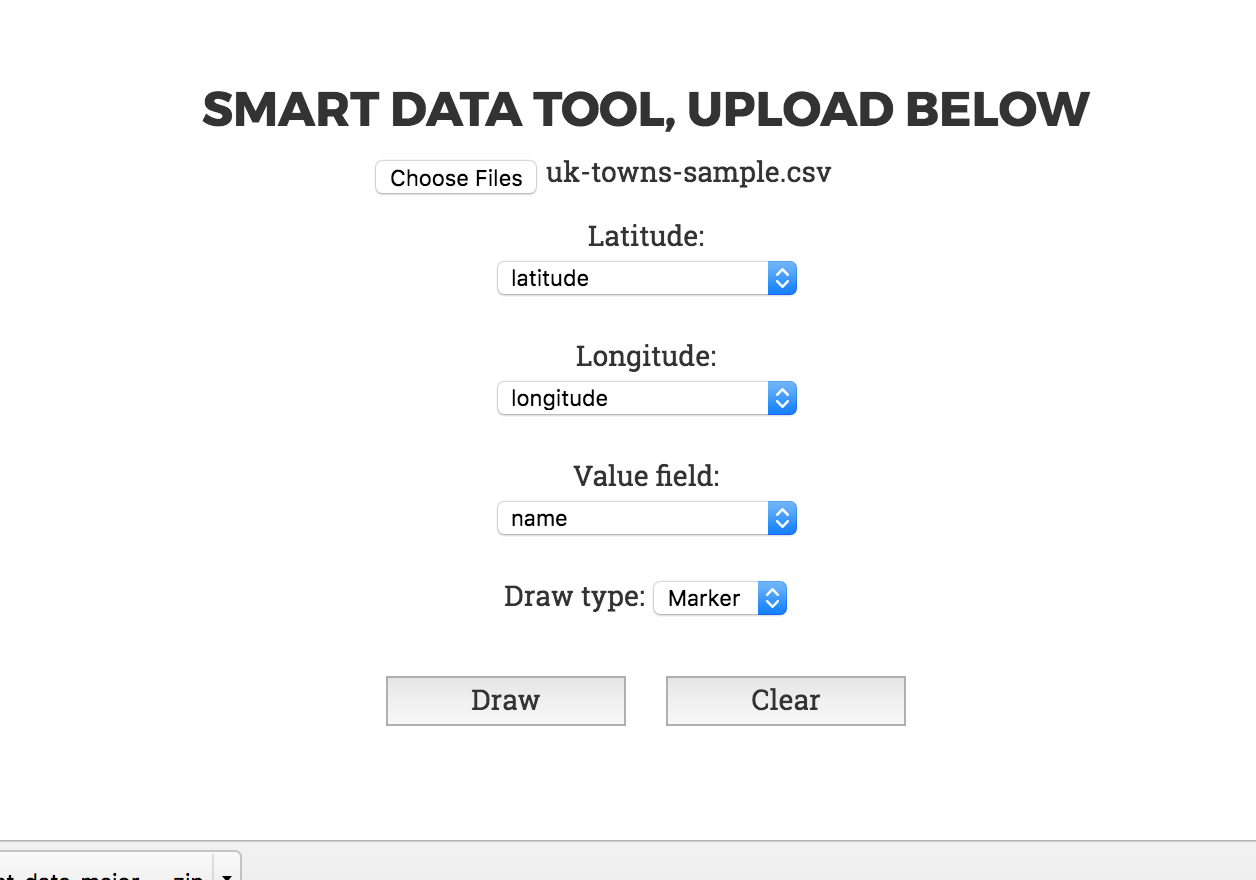
\includegraphics[width=0.4\textwidth]{sdt}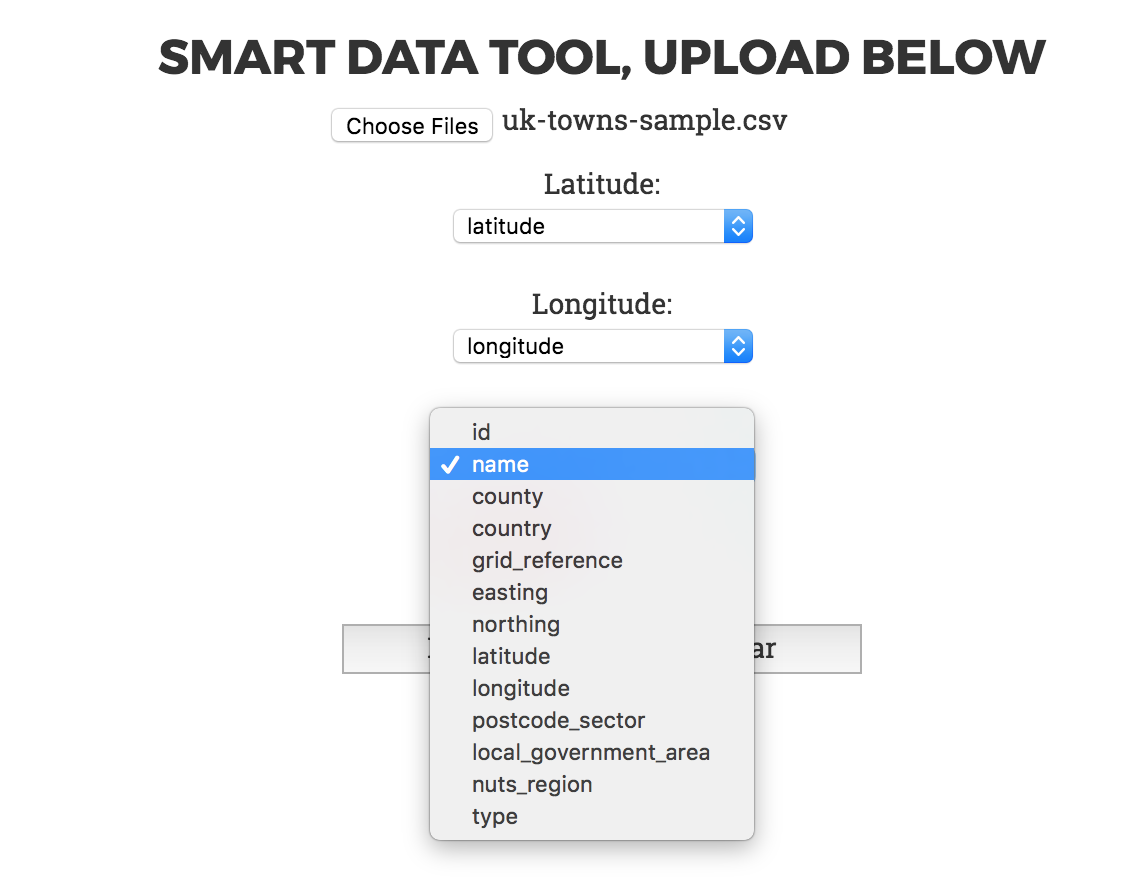
\includegraphics[width=0.4\textwidth]{sdt15}
\caption{Smart Data Tool Town Example}
\label{fig:sdt}
\end{center}
\end{figure}

And Figure \ref{fig:sdt2} shows the result when the uk-towns-sample.csv dataset is drawn with the allergy symptoms heatmap behind.

\begin{figure}[H]
\begin{center}
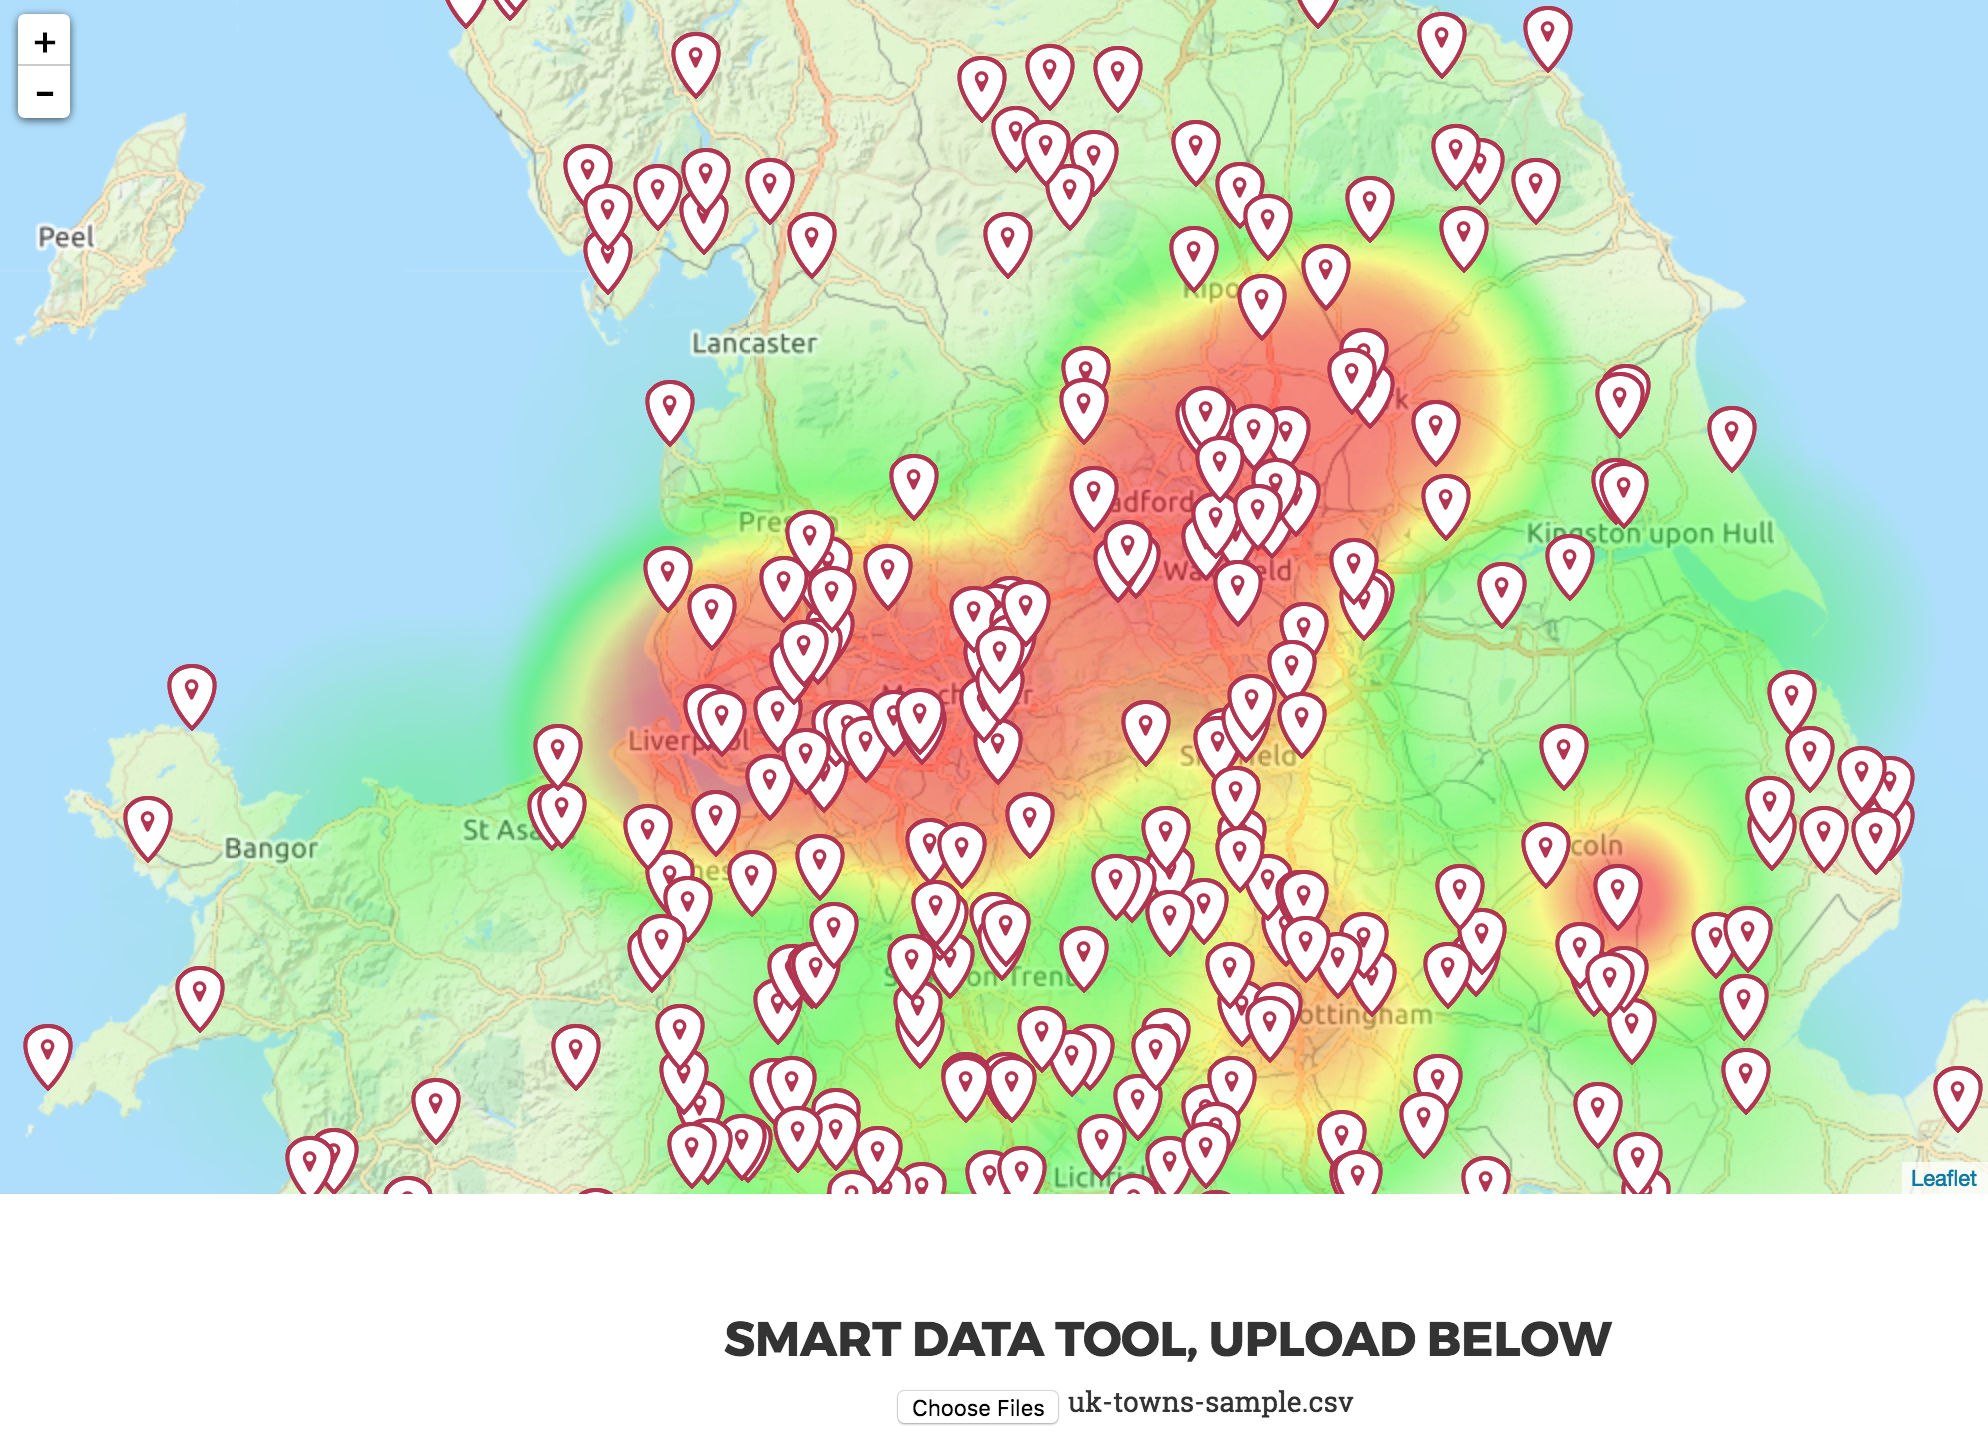
\includegraphics[width=0.4\textwidth]{sdt2}
\caption{Smart Data Tool Town Map}
\label{fig:sdt2}
\end{center}
\end{figure}
\chapter{Testing, Interpretation and Evaluation}
\label{cha:tande}

Chapter 5
\chapter{Conclusion}
\label{cha:conc}

Chapter 6

\bibliography{refs}             % this causes the references to be
                                % listed

\bibliographystyle{alpha}       % this determines the style in which
                                % the references are printed, other
                                % possible values are plain and abbrv
%% Appendices start here
%%\appendix
%%\chapter{Example of operation}

An appendix is just like any other chapter, except that it comes after
the appendix command in the master file.

One use of an appendix is to include an example of input to the system
and the corresponding output.

One way to do this is to include, unformatted, an existing input file. 
You can do this using \verb=\verbatiminput=. In this appendix we
include a copy of the C file \textsf{hello.c} and its output file
\textsf{hello.out}. If you use this facility you should make sure that
the file which you input does not contain \texttt{TAB} characters,
since \LaTeX\ treats each \texttt{TAB} as a single space; you can use
the Unix command \texttt{expand} (see manual page) to expand tabs into
the appropriate number of spaces. 

\section{Example input and output}
\label{sec:inp-eg}
\subsection{Input}
\label{sec:input}
(Actually, this isn't input, it's the source code, but it will do as
an example)

\verbatiminput{hello.c}

\subsection{Output}
\label{sec:output}

\verbatiminput{hello.out}
\subsection{Another way to include code}
You can also use the capabilities of the \texttt{listings} package to
include sections of code, it does some keyword highlighting.

\lstinputlisting[language=C]{hello.c}

% Local Variables: 
% mode: latex
% TeX-master: "report"
% End: 

\end{document}
